
\section{Proposed Methodology}
\label{sec:proposed_methodology}
In this section, we outline the key stages of our research, which consist of three distinct steps designed to address the challenges of handling emerging new classes in changeable data streams. Our proposed approach aims to develop a robust framework capable of tackling these complex challenges through a comprehensive, three-step methodology.
\begin{enumerate}
	\item \textbf{Emerging New Classes:} Our study addresses the widespread issue of emerging new classes in drifted streams using well-known techniques, including concept drift detection and K-means clustering.
	\item \textbf{Drifted Streams:} To address changes in the data distribution, our approach integrates a concept drift detector that dynamically identifies shifts, allowing the model to promptly adapt its classifiers to maintain effectiveness.
	\item \textbf{Classifier Performance:} Classifier Performance: We utilize Dynamic Ensemble Selection (DES) to boost classifier performance. This method involves constructing a pool of classifiers and dynamically choosing the most appropriate one for each new data point, thereby enhancing both accuracy and robustness.
\end{enumerate}
\subsection{Proposed Approach Flow}
\label{proposed_overview}
Our proposed approach is composed of three main phases that work together to manage emerging new classes and drifting data streams effectively:
\begin{enumerate}
	\item \textbf{Dynamic Ensemble Selection:} The initial phase, DES, identifies the most suitable classifier for each incoming data chunk to ensure optimal performance.
	\item \textbf{Drift Detector Phase:} In this phase, the system continuously observes the data stream in real time to detect concept drift, indicating changes in the underlying data distribution.
	\item \textbf{Emerging New Class Identifier Phase:} The final phase identifies unknown classes in drifted streams, creating new classifiers for emerging classes to improve the model's proficiency in accurately classifying new instances.
\end{enumerate}
As depicted in Fig. \ref{fig:proposal_step_1}, DES extracts the current data chunk and utilizes the DES technique to identify the most effective classifiers for that chunk (black box of Fig. \ref{fig:proposal_step_1}). These classifiers are used in the second phase to predict class labels, while drift detectors like ADWIN or DDM monitor for concept drift. If a drift is detected (highlighted by the red rectangle), the chunk is forwarded to the third phase, where new classes are identified (see Fig. \ref{fig:proposal_step_2}). The overall approach is implemented in Algorithm \ref{alg:5_alg_1}, which takes a data stream and a DES Pool threshold as inputs. Key components include training the initial ensemble (Lines 4-6), using DES to select the best classifier for the current chunk (Line 8), detecting drifted chunks (Line 10), creating new classifiers for emerging classes (Line 12), and removing the worst classifier if the DES Pool threshold is exceeded (Lines 14-16).

\subsection{Emerging New Classes Phase Details}
\label{sec:emerging_phase}
In this section we present the Emerging new classes phase details. As shown in Fig.2, The emerging phase contains two primary steps:
\begin{enumerate}
	\item \textbf{Emerging new classes identifier:} The emerging class detection step plays a crucial role in the proposed approach (the black rectangle of Fig. \ref{fig:proposal_step_2}) by utilize the K-means technique to clustering the drifted chunk into a set of clusters. And identifying new emerging classes by evaluating the distances between instances and their nearest class centroid. This process involves comparing the distance between an instance and the nearest class centroid with the maximum distance between class centroids ($d_c$), as described in Eq.\ref{eq:equation_1} and Eq.\ref{eq:equation_2}, where ED represents the Euclidean Distance method and $c_i$, $c_j$ denotes the centroids of the current classes. If the calculated distance ($d_x$) exceeds this threshold ($d_c$), this indicates the presence of a new emerging class, denoted by EC in Eq. \ref{eq:equation_3}; otherwise, it is $P_DES$ (prediction class of the new instance).
	\item \textbf{Adaptive the Emerging classes pool size:} This critical step adapts the pool size based on the emergence rate of new classes and drift distribution, using statistical measures like standard deviation, first derivative, and average historical drift updates.
\end{enumerate}
The Emerging New Classes phase is implemented in Algorithm \ref{alg:5_alg_2}, which utilizes drifted instances and current changes as inputs. Key steps include applying K-means (Line 1), calculating cosine similarity between centroids (Line 2), determining the maximum centroid distance (Line 3), setting the adaptive pool threshold (Lines 4-7), using KNN to find the nearest neighbor (Line 9), storing instances in the emerging pool if the distance exceeds the threshold (Lines 11-12), and creating a new classifier if the pool size surpasses the adaptive limit (Lines 14-17). A simulated scenario is illustrated in Figures  \ref{fig:scenario1} and  \ref{fig:scenario2}. In Fig. \ref{fig:scenario1} (a), the drifted chunk is divided into three clusters using the K-means algorithm. Fig. \ref{fig:scenario1} (b) shows the calculation of the maximum distance between cluster centroids, which serves as a threshold for identifying new classes. The procedure for classifying instances is as follows: when a drifted instance is detected, it is considered a new class if the distance between the instance and its nearest centroid exceeds the maximum inter-centroid distance Fig. \ref{fig:scenario2} (a). If the distance is within the threshold, the instance is classified as a known class Fig. \ref{fig:scenario2} (b).

\begin{figure}[ht]
	\centering
	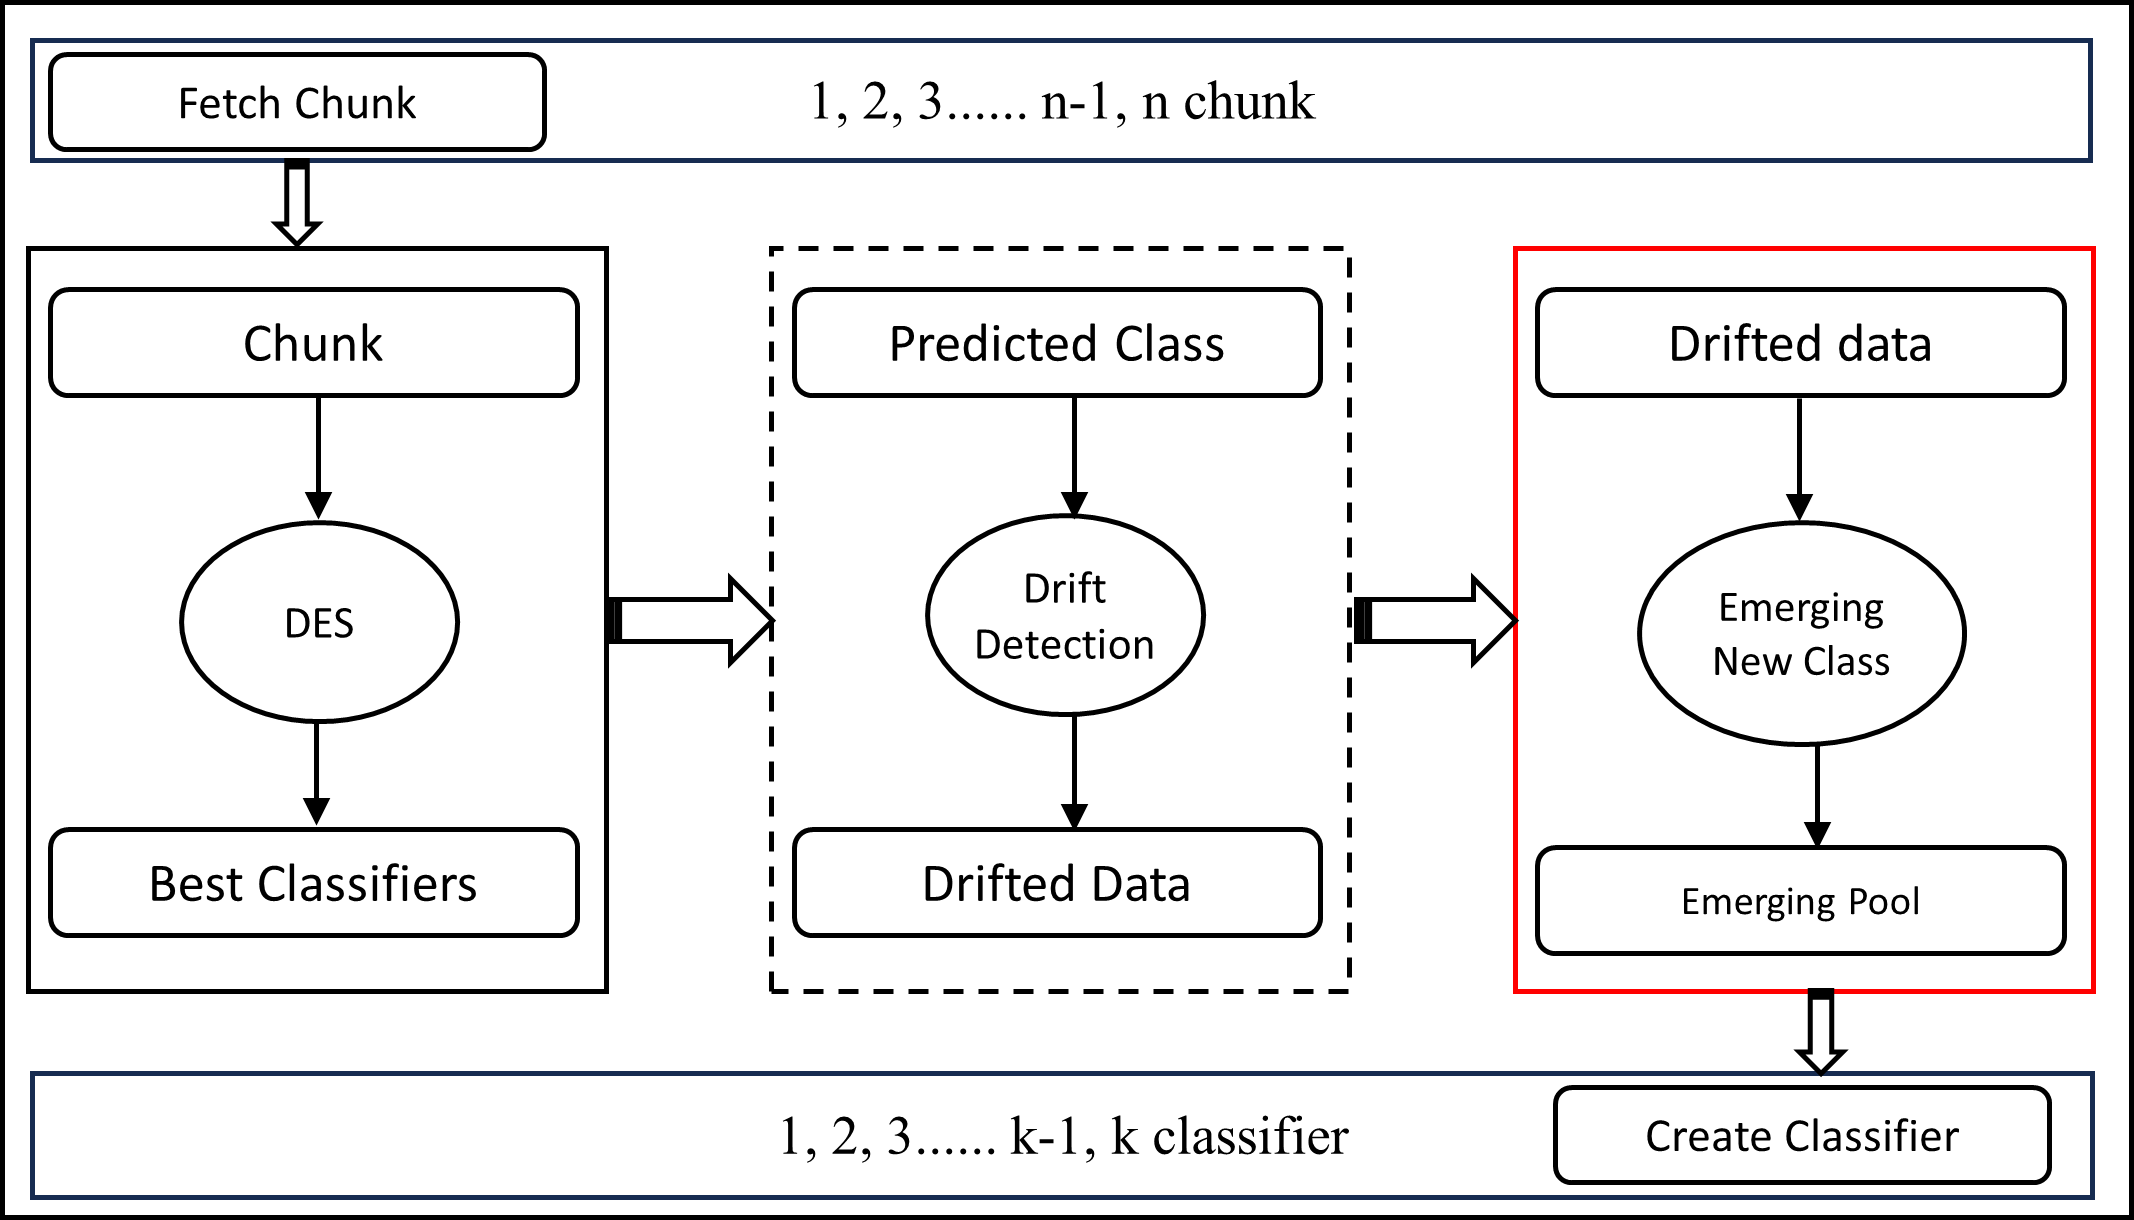
\includegraphics[width=1\linewidth]{5_Emerging/images/pro1.png}
	\caption{Flow of the proposed approach for emerging drifted
	data.}
	\label{fig:proposal_step_1}
\end{figure}

\begin{figure}[ht]
	\centering
	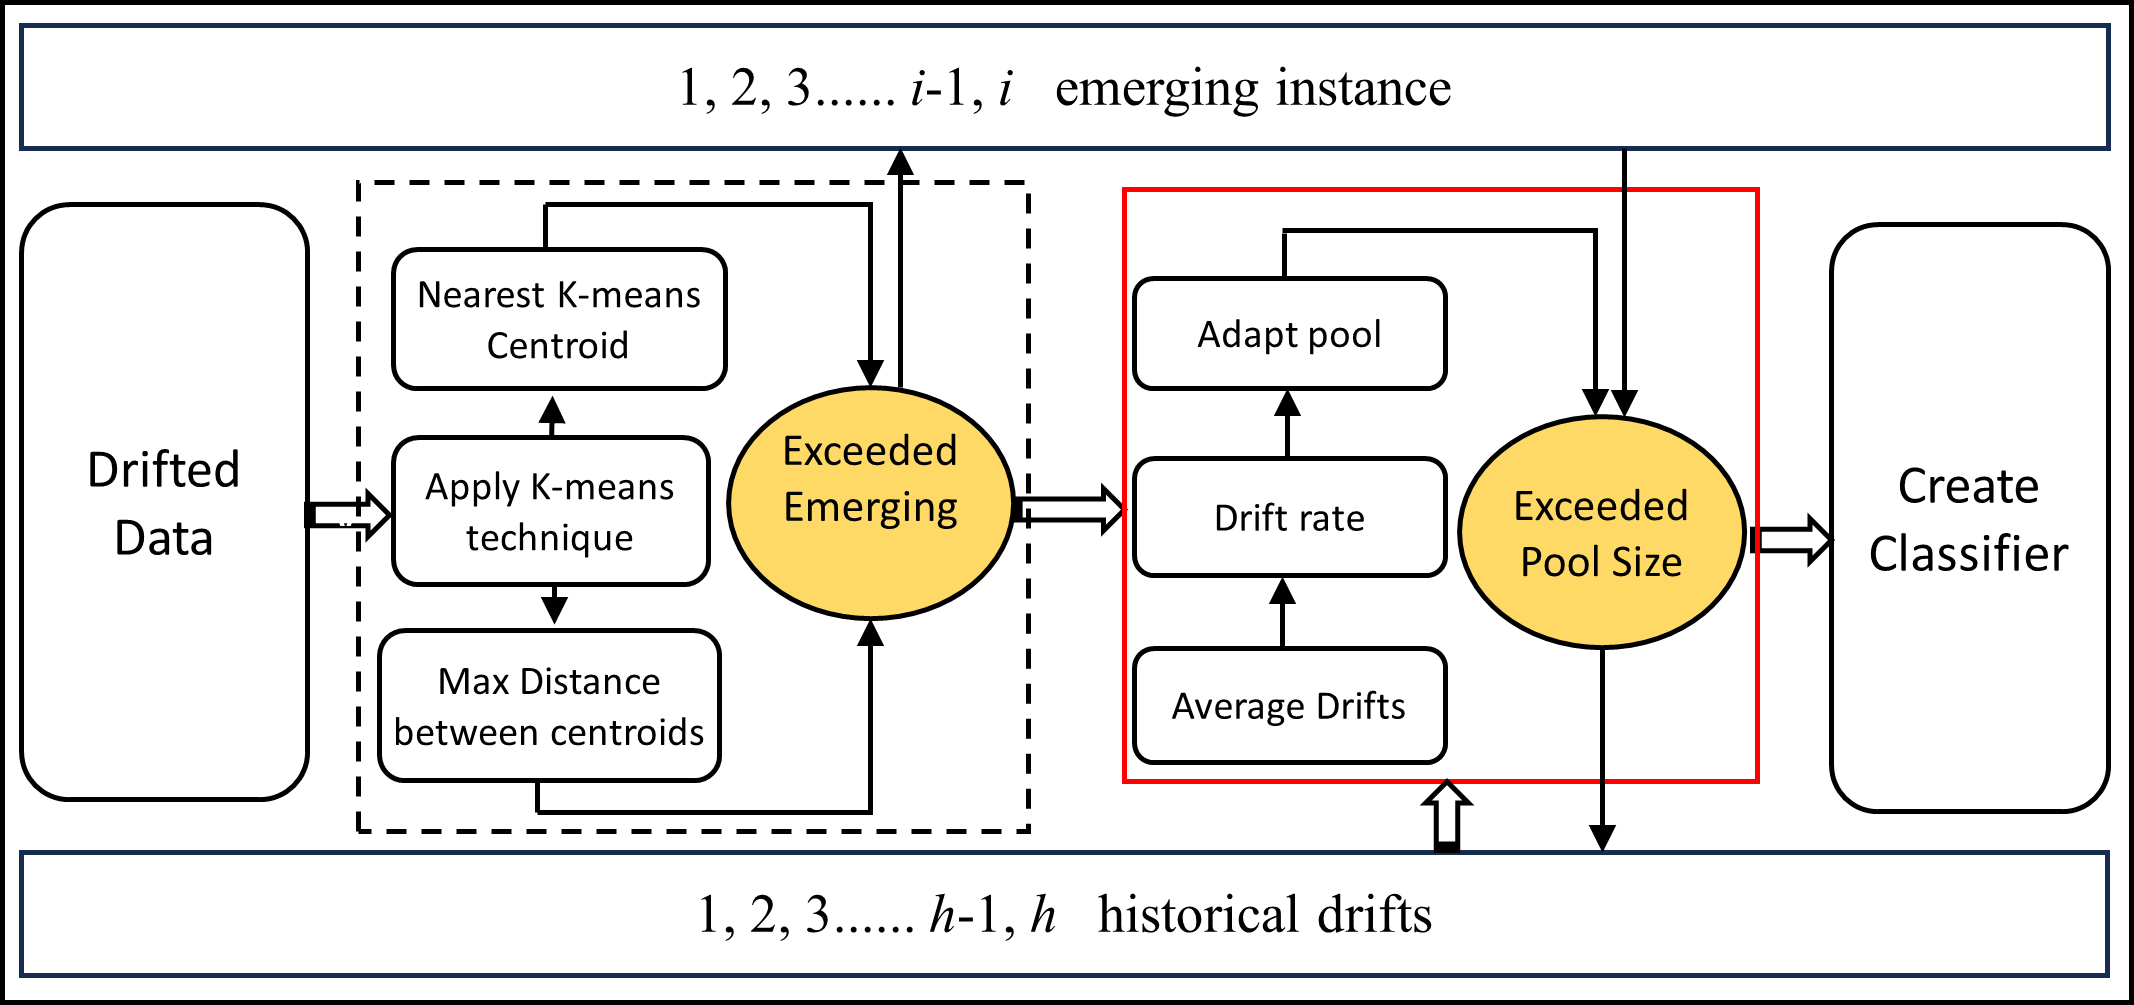
\includegraphics[width=1\linewidth]{5_Emerging/images/pro2.png}
	\caption{Flow of the Emerging Phase.}
	\label{fig:proposal_step_2}
\end{figure}
\begin{figure}[!ht]
    \centering
    \begin{minipage}{0.48\textwidth}
        \centering
        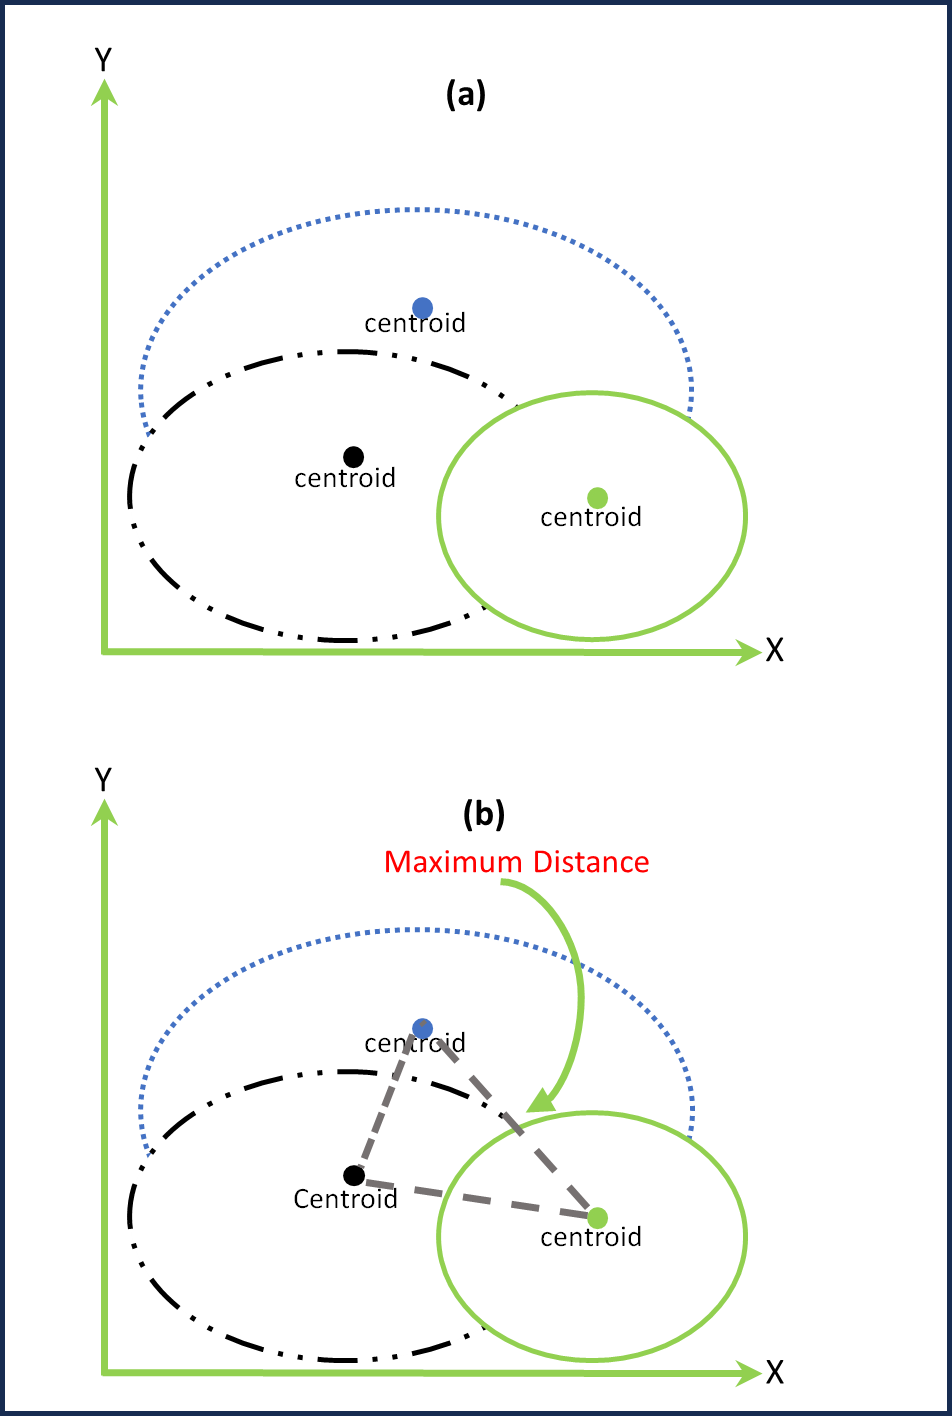
\includegraphics[width=\linewidth]{5_Emerging/images/scenario1.png}
        \caption{Example steps for a dataset with two features (x, y) and three classes (Blue, Black, Green): (a) Use the K-means algorithm to cluster the current chunk. (b) Determine the maximum distance between class centroids.}
        \label{fig:scenario1}
    \end{minipage}
    \hfill
    \begin{minipage}{0.48\textwidth}
        \centering
        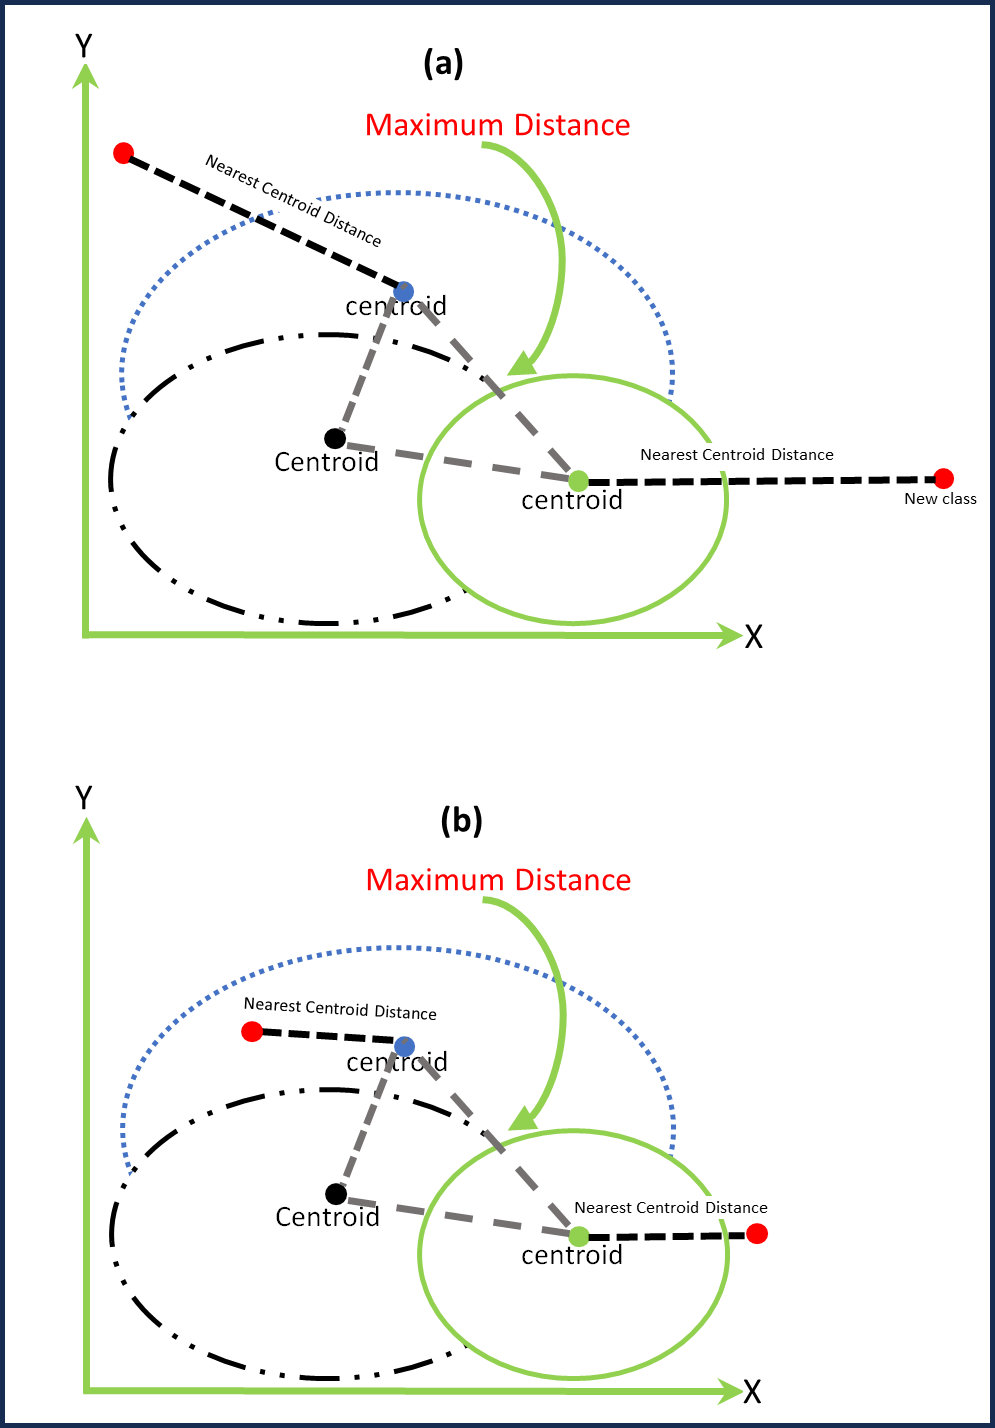
\includegraphics[width=\linewidth]{5_Emerging/images/scenario2.png}
        \caption{Example steps for new points (red points) with two features (x, y): (a) Identify new incoming instances (represented by red points) as potential new classes. (b) Determine whether the new instance is part of a nearby existing class or belongs to an emerging new class.}
        \label{fig:scenario2}
    \end{minipage}
\end{figure}



\begin{equation}
	\label{eq:equation_1}
	d_c = \arg\max_d \sum_{i=1}^{i} \sum_{j=i+1}^{i}  ED(c_i, c_j)
\end{equation}

\begin{equation}
	\label{eq:equation_2}
	d_x = \arg\min_i \sum_{i=1}^{i} ED(x, c_i)
\end{equation}

\begin{equation}
	\label{eq:equation_3}
	p=
	\begin{cases}
		EC & \text{if } d_x > d_c \\
		P_{DES} & \text{otherwise}
	\end{cases}
\end{equation}


\begin{algorithm}[h]
	\SetAlgoLined
	\DontPrintSemicolon
	\KwIn{data stream, classifier threshold $\kappa$}
	\KwData{current chunk $\emph{a}$, classifier $\emph{k}$, classifiers pool $\Psi$, drifted pool $\psi$}
	\KwOut{prediction $\emph{p}$}
	$\psi \gets \phi$\;
	$\Psi \gets \phi$\;
	\For{stream has chunk}{
		\eIf{$\emph{a}$ is the first chunk}{
			$\emph{k} \gets \text{trainingNewClassifier}(\emph{a})$\;
			$\emph{P} \gets \text{getPrediction}(\emph{a}, \emph{k})$\;
		}{
			$\emph{k} \gets \text{DES}(\emph{a}, \Psi)$\;
			$\emph{P} \gets \text{getPrediction}(\emph{a}, \emph{k})$\;
			$\psi \gets \text{conceptDriftDetector}(\emph{P})$\;

			\If{$\psi > 0$}{
				$\emph{k} \gets \text{utilize } \emph{a} \text{ and } \psi \text{ to get new classes according to Algorithm \ref{alg:5_alg_2}}$\;
				$\Psi \gets \Psi + \emph{k}$\;
				\If{$|\Psi| > \kappa$}{
					$\text{removeWorstClassifier}(\emph{a})$\;
				}
				$\emph{p} \gets \text{getPrediction}(\emph{a}, \emph{k})$\;
			}
		}
	}
	\Return{$\emph{p}$}\;
	\caption{Proposed approach algorithm for emerging drifted
	data streams.}
	\label{alg:5_alg_1}
\end{algorithm}

\begin{algorithm}[h]
	\SetAlgoLined
	\DontPrintSemicolon
	\KwIn{current chunk $\emph{a}$, drifted pool $\psi$, historical drifts $\emph{h}$}
	\KwData{current chunk $\emph{a}$, classifier $\emph{k}$, Stream Emerging New Classes $\text{SENC}$, $\text{SENC Pool } \Psi$, K-means centroids $\lambda$, centroid distance $\Phi$, maximum centroid distance $\emph{dc}$, chunk distance $\emph{i}$, Nearest neighbor $\emph{n}$, historical drifts $\emph{h}$, average historical drifts $\mu$}
	\KwOut{classifier $\emph{k}$}
	$\lambda \gets \text{apply Kmeans}(\emph{a})$\;
	$\Phi \gets \text{apply cosine similarity}(\lambda)$\;
	$\emph{dc} \gets \max(\Phi)$\;
	$\mu \gets \frac{\sum \emph{h}}{|\emph{h}|}$\;
	$\sigma \gets \text{std}(\psi)$\;
	$\Delta \gets \text{first derivative}(\emph{h})$\;
	$\text{threshold} \gets \mu + \Delta \times \sigma$\;

	\For{$\psi$ has instance}{
		$\emph{n} \gets \text{apply KNN}(\lambda, \emph{i})$\;
		$\emph{d} \gets \text{apply cosine similarity}(\emph{i}, \emph{n})$\;
		\If{$\emph{d} \geq \emph{dc}$}{
			$\Psi \gets \Psi + \emph{i}$\;
		}
		\If{$|\Psi| \geq \text{threshold}$}{
			$\emph{k} \gets \text{trainingNewClassifier}(\emph{a})$\;
			$\emph{h} \gets \emph{h} + \psi$\;
			$\Psi \gets \phi$\;
		}
	}
	\Return{$\emph{k}$}\;
	\caption{Flow of the Emerging Phase.}
	\label{alg:5_alg_2}

\end{algorithm}